\documentclass[9pt,twocolumn,twoside]{opticajnl}
\journal{opticajournal} % use for journal or Optica Open submissions

% See template introduction for guidance on setting shortarticle option
\setboolean{shortarticle}{true}
% true = letter/tutorial
% false = research/review article

% ONLY applicable for journal submission shortarticle types:
% When \setboolean{shortarticle}{true}
% then \setboolean{memo}{true} will print "Memorandum" on title page header
% Otherwise header will remain as "Letter"
% \setboolean{memo}{true}

\usepackage{lineno}
\linenumbers % Turn off line numbering for Optica Open preprint submissions.
\raggedbottom % Leave empty space at the bottom of a column instead of stretching the space between paragraphs
\setlength{\textfloatsep}{8pt plus 2pt minus 2pt} % Space between a float at the top of a column and the text
\setlength{\intextsep}{8pt plus 2pt minus 2pt}    % Space around a float placed inside the text ([H])

\title{TITTLE HERE}

\author[1,*]{Amilcar Abdiel Díaz García}

\affil[1]{Department of Civil and Environmental Engineering, University of Alberta, Edmonton, AB, Canada}

\affil[*]{adiazgar@ualberta.ca}

\begin{abstract}
% PENDIENTE: resumen
\end{abstract}

\setboolean{displaycopyright}{false} % Do not include copyright or licensing information in submission.

\begin{document}

\maketitle

\section{Introducción}
% PENDIENTE: introducción

\section{Metodología}

La idea principal de este estudio es que, si un modelo de machine learning es capaz de aprender a predecir las frecuencias naturales del puente sano bajo condiciones ambientales específicas, las mediciones del monitoreo continuo pueden compararse con esa predicción para generar alertas y detectar el daño lo antes posible. Para esto, también se tiene en cuenta la dispersión dada por la estimación de las frecuencias naturales y por la variabilidad del tráfico, que pueden suponerse normales. La Fig.~\ref{fig:method} resume el método utilizado.

\begin{figure}[H]
\centering
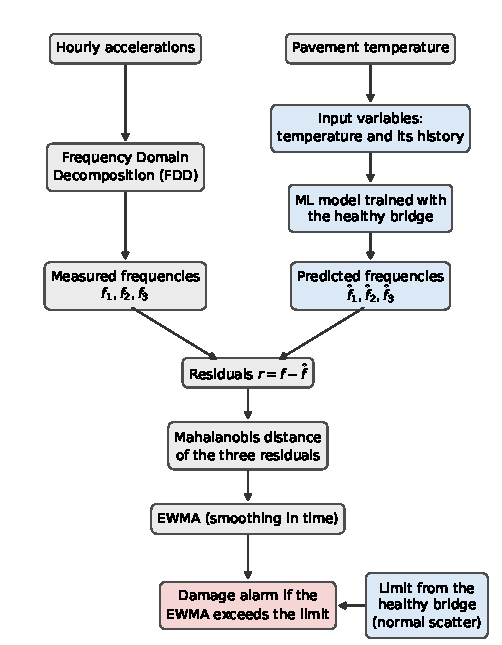
\includegraphics[width=\linewidth]{figures/method_flowchart}
\caption{Esquema del método. En azul, lo que se obtiene con las mediciones del puente sano.}
\label{fig:method}
\end{figure}

\subsection{Datos}

Para este estudio se utilizaron los datos medidos en el puente Z24, en Suiza. Estas mediciones fueron realizadas por el grupo de Mecánica Estructural de la KU Leuven (Bélgica) y los datos se publicaron en \cite{Peeters2001}.

El Z24 es un puente de concreto postensado de tres vanos, como se observa en la Fig.~\ref{fig:z24-bridge}, donde también se ilustran las posiciones en las que se colocaron los sensores.

\begin{figure}[ht]
\centering
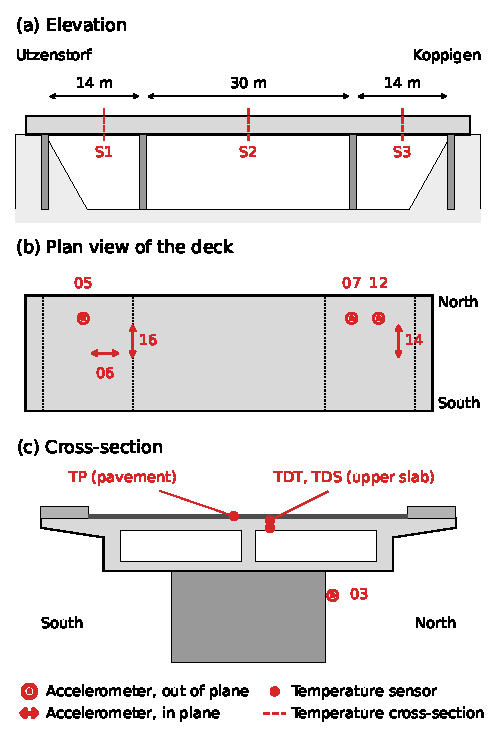
\includegraphics[width=\linewidth]{figures/bridge_sensors}
\caption{Puente Z24 y posición de los sensores utilizados en este estudio (esquema sin escala, posiciones aproximadas): (a) elevación, (b) planta del tablero y (c) sección transversal.}
\label{fig:z24-bridge}
\end{figure}

Las mediciones tomadas por el grupo de investigación incluyen las aceleraciones del puente, la temperatura del aire, la humedad relativa, la lluvia, la velocidad y dirección del viento, la temperatura del suelo junto a las pilas y los estribos, y la temperatura en distintos puntos de la estructura (pavimento, losas superior e inferior, almas y veredas). Estas mediciones se hicieron durante casi un año, del 10 de noviembre de 1997 al 10 de septiembre de 1998. Durante los primeros nueve meses el puente estuvo sano. Después, a partir del 11 de agosto de 1998, se le aplicaron daños progresivos y se siguieron tomando las mismas mediciones sobre el puente dañado.

Para este estudio solo se tomaron en cuenta las aceleraciones, la temperatura del pavimento y la temperatura de la losa superior para analizar el efecto de los cambios de temperatura en las propiedades dinámicas del puente. 

A partir de las aceleraciones medidas se obtuvieron las frecuencias naturales de los tres primeros modos del puente, aplicando el método de descomposición en el dominio de la frecuencia (FDD, \emph{Frequency Domain Decomposition}) \cite{Brincker2001}.

Como se observa en la Fig.~\ref{fig:frequency-temperature}, los cambios de temperatura pueden afectar significativamente las frecuencias naturales del puente. Por esta razón, en ciudades como Edmonton, Alberta, que cuentan con un rango de temperaturas muy amplio a lo largo del año, no se puede establecer un único umbral de frecuencias naturales para determinar si un puente está sano o dañado. Por ello, es necesario analizar la relación que existe entre las frecuencias naturales y la temperatura de la estructura. Además, en la Fig.~\ref{fig:frequency-temperature} se puede observar que existe una relación aparentemente bilineal entre las frecuencias naturales y la temperatura del pavimento con un quiebre justo en $0\,^\circ$C. Esto refuerza lo encontrado por Peeters y De Roeck \cite{Peeters2001}, quienes atribuyeron este comportamiento al aumento de la rigidez de la capa de asfalto cuando se congela.

\begin{figure}[H]
\centering
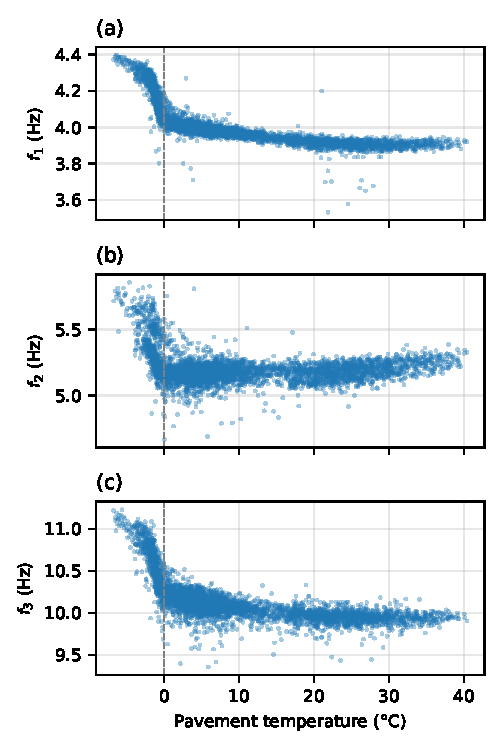
\includegraphics[width=\linewidth]{figures/frequency_vs_temperature}
\caption{Frecuencia natural frente a la temperatura del pavimento, puente sano (10.11.1997 al 04.08.1998): (a) modo 1, (b) modo 2 y (c) modo 3. La línea discontinua marca $0\,^\circ$C.}
\label{fig:frequency-temperature}
\end{figure}

Para este estudio se tomaron los datos del puente Z24 ya que cubren un amplio rango de condiciones climáticas. La Tabla~\ref{tab:temperature-range} muestra el rango de temperaturas medidas con el puente sano, por estación. Como se observa, durante el invierno la temperatura del pavimento estuvo bajo $0\,^\circ$C en un 38\% de las mediciones. 

\begin{table}[H]
\centering
\caption{\bf Temperaturas medidas con el puente sano, por estación (10.11.1997 al 04.08.1998)}
\small
\setlength{\tabcolsep}{3pt}
\begin{tabular}{lrrrrrrrr}
\hline
 & & \multicolumn{3}{c}{Pavimento ($^\circ$C)} & \multicolumn{3}{c}{Losa sup. ($^\circ$C)} & $<0\,^\circ$C \\
Estación & $n$ & Mín. & Media & Máx. & Mín. & Media & Máx. & (\%) \\
\hline
Otoño & 490 & $-0.3$ & 3.5 & 8.2 & $-0.5$ & 3.2 & 7.2 & 3.7 \\
Invierno & 2043 & $-6.7$ & 2.0 & 13.9 & $-5.4$ & 1.9 & 9.3 & 38.0 \\
Primavera & 1227 & $-0.5$ & 10.4 & 31.0 & 0.1 & 8.4 & 22.0 & 0.3 \\
Verano & 1061 & 15.0 & 26.3 & 40.4 & 15.0 & 22.5 & 32.0 & 0.0 \\
\hline
Total & 4821 & $-6.7$ & 9.6 & 40.4 & $-5.4$ & 8.2 & 32.0 & 16.6 \\
\hline
\end{tabular}
  \label{tab:temperature-range}

\smallskip
\footnotesize
$n$: número de mediciones horarias. La última columna es el porcentaje de mediciones con la temperatura del pavimento bajo $0\,^\circ$C. Otoño: desde el 10.11.1997; verano: hasta el 04.08.1998.
\end{table}

\subsection{Limpieza de datos}

La Tabla~\ref{tab:accelerometers} resume los acelerómetros utilizados en este estudio. De los 16 acelerómetros instalados, ocho no registraron información durante las mediciones, por lo que fueron descartados. También se descartó el acelerómetro 10, ya que en más de la mitad de las mediciones su señal se mantuvo fija en un valor constante (sin vibración).

\begin{table}[H]
\centering
\caption{\bf Acelerómetros utilizados en este estudio}
\small
\begin{tabular}{lll}
\hline
Canal & Ubicación & Dirección \\
\hline
03 & Pila, parte superior & Longitudinal \\
05 & Tablero, borde norte, lado Utzenstorf & Vertical \\
06 & Tablero, lado Utzenstorf & Longitudinal \\
07 & Tablero, borde norte, lado Koppigen & Vertical \\
12 & Tablero, borde norte, lado Koppigen & Vertical \\
14 & Tablero, extremo Koppigen & Transversal \\
16 & Tablero, lado Utzenstorf & Transversal \\
\hline
\end{tabular}
  \label{tab:accelerometers}
\end{table}

Durante el estudio hubo un periodo en el que se preparó el puente para aplicarle los daños progresivos. En ese periodo, la frecuencia natural del modo 2 disminuyó respecto a las frecuencias que se venían midiendo normalmente en ese mismo rango de temperaturas (Fig.~\ref{fig:damage-preparation}). Por ello, se decidió descartar las frecuencias naturales estimadas del 5 al 11 de agosto de 1998, ya que su dispersión no representa la variación normal del puente bajo condiciones ambientales y de tráfico normales.

\begin{figure}[H]
\centering
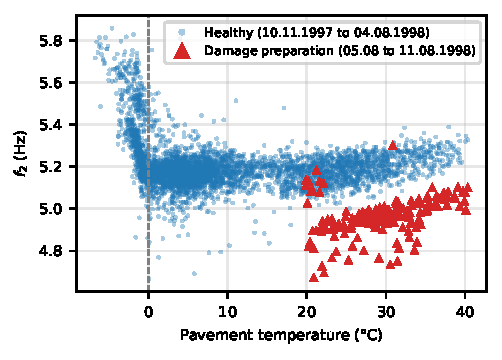
\includegraphics[width=\linewidth]{figures/damage_preparation_f2}
\caption{Frecuencia natural del modo 2 frente a la temperatura del pavimento: puente sano (10.11.1997 al 04.08.1998) y periodo de preparación para los daños (05.08 al 11.08.1998). La línea discontinua marca $0\,^\circ$C.}
\label{fig:damage-preparation}
\end{figure}

\subsection{División de los datos y validación}
\label{sec:data-split}

Los modelos de machine learning se probaron tanto con el puente sano, donde no deberían indicar daño, como con el puente dañado, donde deberían indicarlo lo antes posible. Considerando esto, el dataset de prueba está compuesto por las mediciones del puente dañado, un periodo de mediciones del puente sano justo antes de la preparación para los daños y otro periodo de mediciones del puente sano en invierno, que incluye temperaturas bajo $0\,^\circ$C.

Para la validación cruzada, el dataset de entrenamiento y validación se dividió en 5 folds. Estos folds no se formaron al azar con mediciones sueltas, ya que las frecuencias naturales de dos mediciones consecutivas son muy parecidas y el propósito es que el modelo pueda predecir las frecuencias naturales del puente sano en días que no haya visto antes. Para lograrlo, los folds se formaron con bloques de una semana, como se muestra en la Fig.~\ref{fig:data-split}.

La Tabla~\ref{tab:data-split} resume la división de los datos utilizada para la construcción y la prueba de los modelos de machine learning. De esta manera se garantiza que el modelo sea entrenado y validado para las diferentes condiciones de temperatura medidas y también se puede probar tanto para temperaturas de verano, como para temperaturas de invierno con mediciones que el modelo no vio durante la etapa de entrenamiento y validación.

\begin{figure}[H]
\centering
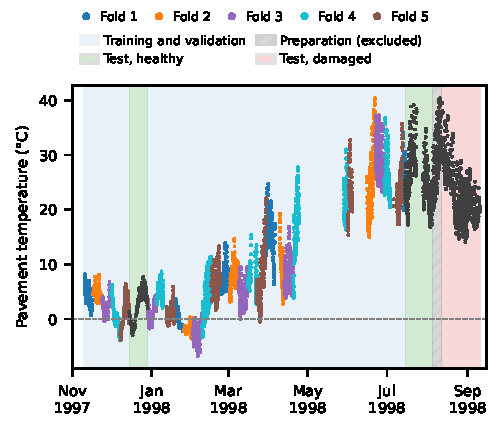
\includegraphics[width=\linewidth]{figures/data_split}
\caption{División de los datos sobre la temperatura del pavimento. Las áreas sombreadas marcan los bloques: entrenamiento y validación, pruebas con el puente sano en invierno (15.12 al 28.12.1997) y en verano (15.07 al 04.08.1998), preparación para los daños (excluida, 05.08 al 11.08.1998) y prueba con el puente dañado (desde el 11.08.1998). El color de los puntos indica el fold de cada medición (bloques de una semana repartidos por turnos en 5 folds). La línea discontinua marca $0\,^\circ$C.}
\label{fig:data-split}
\end{figure}

\begin{table}[H]
\centering
\caption{\bf Mediciones de cada conjunto y de cada fold}
\small
\begin{tabular}{lrr}
\hline
Conjunto & Mediciones & Bajo $0\,^\circ$C \\
\hline
Fold 1 & 677 & 101 \\
Fold 2 & 650 & 109 \\
Fold 3 & 955 & 207 \\
Fold 4 & 833 & 120 \\
Fold 5 & 818 & 106 \\
Entrenamiento y validación & 3933 & 643 \\
\hline
Prueba, puente sano (invierno) & 320 & 82 \\
Prueba, puente sano (verano) & 324 & 0 \\
Preparación (excluida) & 158 & 0 \\
Prueba, puente dañado & 494 & 0 \\
\hline
\end{tabular}
  \label{tab:data-split}

\smallskip
\footnotesize
Mediciones con las tres frecuencias naturales y las temperaturas del pavimento y de la losa superior; en la preparación se cuentan todas las mediciones. Bajo $0\,^\circ$C: temperatura del pavimento.
\end{table}

\subsection{Modelo del comportamiento sano}

Debido a la relación bilineal observada en la Fig.~\ref{fig:frequency-temperature}, se inició probando con un modelo lineal con dos pendientes, una sobre $0\,^\circ$C y otra bajo $0\,^\circ$C, que relacionaba las frecuencias naturales del puente sano con la temperatura del pavimento en cada medición. Los residuos de ese modelo se analizaron para decidir si el modelo era capaz de predecir correctamente las frecuencias naturales del puente sano o si había que considerar otras variables o cambiar de modelo. En cada medición, el residuo es la diferencia entre la frecuencia natural medida y la frecuencia natural predicha por el modelo:
\begin{equation}
r_{m,i} = f_{m,i} - \hat{f}_{m,i},
\label{eq:residual}
\end{equation}
donde $r_{m,i}$ es el residuo del modo $m$ en la medición $i$, $f_{m,i}$ es la frecuencia natural medida y $\hat{f}_{m,i}$ es la frecuencia natural predicha.

Después, se agregaron otras variables para representar el efecto del enfriamiento y del calentamiento progresivo de la estructura (Sección~\ref{sec:input-variables}). Luego, con esas variables, se probaron modelos más complejos que el lineal (Sección~\ref{sec:candidate-models}). Finalmente, se eligió un modelo para cada frecuencia natural con el criterio de la Sección~\ref{sec:selection-criterion}.

\subsubsection{Variables de entrada}
\label{sec:input-variables}

Considerando que no toda la estructura tiene la misma temperatura en todos sus puntos y solamente se contaba con mediciones de temperatura en la superficie del pavimento y en la losa superior, se agregaron variables que representan el enfriamiento y el calentamiento progresivo de la estructura. La primera fue el promedio de la temperatura del pavimento de las últimas 6, 12 y 24 horas, ya que Peeters y De Roeck \cite{Peeters2001} encontraron que un modelo que incluye las temperaturas de las horas anteriores predice mejor las frecuencias naturales del Z24 que un modelo que solo usa la temperatura actual. Este promedio se calculó como
\begin{equation}
\bar{T}_{w,i} = \frac{1}{n_{w,i}} \sum_{j\,:\; t_i - w < t_j \le t_i} T_j,
\label{eq:moving-average}
\end{equation}
donde $\bar{T}_{w,i}$ es el promedio de las últimas $w$ horas en la medición $i$, $T_j$ y $t_j$ son la temperatura y la hora de la medición $j$, y $n_{w,i}$ es el número de mediciones en las últimas $w$ horas.

La segunda fue un índice de congelamiento, que acumula la temperatura multiplicada por el tiempo:
\begin{equation}
I_i = \max\left(0,\; I_{i-1} - T_i\,\Delta t_i\right),
\label{eq:freezing-index}
\end{equation}
donde $I_i$ es el índice de congelamiento ($^\circ$C$\cdot$h) en la medición $i$ y $\Delta t_i$ son las horas desde la medición anterior. De esta manera, el índice crece mientras la temperatura está bajo $0\,^\circ$C, disminuye con el deshielo y nunca es negativo.

La Tabla~\ref{tab:feature-sets} resume los conjuntos de variables con los que se probaron los modelos.

\begin{table}[H]
\centering
\caption{\bf Conjuntos de variables de entrada}
\small
\begin{tabular}{ll}
\hline
Conjunto & Variables \\
\hline
Bilineal & $T$, $\min(T,0)$ \\
Historia térmica & $T$, $\bar{T}_6$, $\bar{T}_{12}$, $\bar{T}_{24}$, $h$ \\
Físico & $T$, $\bar{T}_{24}$, $\min(T,0)$, $\sqrt{I}$ \\
\hline
\end{tabular}
  \label{tab:feature-sets}

\smallskip
\footnotesize
$T$: temperatura del pavimento; $\bar{T}_w$: promedio de las últimas $w$ horas (Ec.~\eqref{eq:moving-average}); $\min(T,0)$: igual a $T$ bajo $0\,^\circ$C e igual a 0 sobre $0\,^\circ$C; $h$: horas seguidas bajo $0\,^\circ$C; $I$: índice de congelamiento (Ec.~\eqref{eq:freezing-index}).
\end{table}

\subsubsection{Modelos candidatos}
\label{sec:candidate-models}

Los modelos se probaron en orden de complejidad, de manera que cada modelo agrega algo que el anterior no puede hacer. La regresión lineal se probó con los tres conjuntos de variables de la Tabla~\ref{tab:feature-sets}, y los demás modelos, con los conjuntos Historia térmica y Físico.

El primer modelo fue la regresión lineal, en la que la frecuencia natural predicha es una suma ponderada de las variables de entrada:
\begin{equation}
\hat{f} = \theta_0 + \sum_{j=1}^{p} \theta_j x_j,
\label{eq:linear}
\end{equation}
donde $x_j$ son las $p$ variables del conjunto y $\theta_j$ son los parámetros, que se ajustan por mínimos cuadrados. Es el modelo más simple y sus parámetros se pueden interpretar directamente. Por ejemplo, con el conjunto Bilineal, el parámetro de $\min(T,0)$ es el cambio de pendiente bajo $0\,^\circ$C.

Sin embargo, cuando las variables de entrada se mueven juntas, como la temperatura del pavimento y sus promedios, los parámetros de la regresión lineal pueden volverse muy grandes e inestables. Por ello, el segundo modelo fue una regresión lineal regularizada (Ridge), que agrega al ajuste una penalización de los parámetros grandes:
\begin{equation}
\min_{\boldsymbol{\theta}} \; \sum_{i=1}^{n} \left(f_i - \hat{f}_i\right)^2 + \alpha \sum_{j=1}^{p} \theta_j^2,
\label{eq:ridge}
\end{equation}
donde $n$ es el número de mediciones y el hiperparámetro $\alpha$ controla la penalización. El modelo tiene la misma forma de la Ec.~\eqref{eq:linear}; solo cambia la forma de ajustar sus parámetros.

Los dos modelos anteriores solo pueden representar la forma que ya tienen sus variables de entrada. Por ello, el tercer modelo fue una regresión de vectores de soporte con kernel RBF (SVR, \emph{Support Vector Regression}; RBF, \emph{Radial Basis Function}), que ajusta una curva suave sin imponer su forma:
\begin{equation}
\hat{f}(\mathbf{x}) = b + \sum_{i} a_i \exp\left(-\gamma \lVert \mathbf{x} - \mathbf{x}_i \rVert^2\right),
\label{eq:svr}
\end{equation}
donde $\mathbf{x}$ es el vector de variables de entrada, $\mathbf{x}_i$ son mediciones del entrenamiento, $a_i$ y $b$ son parámetros que se ajustan y $\gamma$ controla qué tan local es cada término. Además, los errores menores que $\varepsilon$ no se penalizan y $C$ controla cuánto se penalizan los demás.

Finalmente, como la curva del SVR es suave, puede tener dificultad para seguir cambios bruscos como los que produce el congelamiento. Por ello, el cuarto modelo fue un random forest, que promedia las predicciones de $B$ árboles de regresión:
\begin{equation}
\hat{f}(\mathbf{x}) = \frac{1}{B} \sum_{b=1}^{B} h_b(\mathbf{x}),
\label{eq:random-forest}
\end{equation}
donde $h_b$ es el árbol $b$, entrenado con una muestra aleatoria de las mediciones, y $B = 200$. Cada árbol divide las mediciones con umbrales sobre las variables, por lo que puede representar cambios bruscos; sin embargo, no puede predecir valores fuera del rango del entrenamiento.

Los hiperparámetros de cada modelo ($\alpha$; $C$, $\gamma$ y $\varepsilon$; y el mínimo de mediciones por hoja y el número de variables por división del random forest) se ajustaron con la validación cruzada de la Sección~\ref{sec:data-split}. En la regresión lineal regularizada y en el SVR, las variables se estandarizaron con la media y la desviación estándar de los folds de ajuste.

\subsubsection{Criterio de selección}
\label{sec:selection-criterion}

Para comparar los modelos se utilizó la raíz del error cuadrático medio (RMSE, \emph{Root Mean Square Error}) de la validación cruzada:
\begin{equation}
\text{RMSE} = \sqrt{\frac{1}{n} \sum_{i=1}^{n} r_i^2},
\label{eq:rmse}
\end{equation}
donde $r_i$ es el residuo (Ec.~\eqref{eq:residual}) de la medición $i$, calculado con el modelo entrenado sin el fold de esa medición, y $n$ es el número de mediciones. De esta manera, cada medición se evalúa con un modelo que no vio su semana. El RMSE se calculó por separado para cada frecuencia natural, por lo que se eligió un modelo para cada una.

Como el RMSE cambia de un fold a otro, un modelo con un RMSE un poco menor no es necesariamente mejor. Por ello, se aplicó la regla de un error estándar: entre los modelos cuyo RMSE no supera al menor RMSE por más de un error estándar, se eligió el más simple. Es decir, se eligió el modelo más simple que cumple
\begin{equation}
\text{RMSE}_j \le \text{RMSE}_{\min} + \frac{s_{\min}}{\sqrt{k}},
\label{eq:one-se}
\end{equation}
donde $\text{RMSE}_j$ es el RMSE del modelo $j$, $\text{RMSE}_{\min}$ es el menor RMSE de todos los modelos, $s_{\min}$ es la desviación estándar del RMSE de ese modelo entre los folds y $k = 5$ es el número de folds. El orden de simplicidad sigue la escalera de la Sección~\ref{sec:candidate-models}: regresión lineal, regresión lineal regularizada, SVR y random forest; con el mismo modelo, el conjunto con menos variables se consideró más simple.

\subsection{Sistema de detección}
\label{sec:detection-system}

Una vez elegido el modelo de cada frecuencia natural, los residuos (Ec.~\eqref{eq:residual}) se utilizaron para detectar el daño, siguiendo los pasos de la Fig.~\ref{fig:method}. Si el puente está sano, los residuos solo representan la dispersión normal que el modelo no logra explicar; si el puente se daña, las frecuencias medidas se alejan de las predichas y los residuos aumentan.

Como el daño puede afectar a las tres frecuencias naturales de manera distinta, los tres residuos de cada medición se combinaron en un solo índice de daño con la distancia de Mahalanobis:
\begin{equation}
d_i = \sqrt{\left(\mathbf{r}_i - \boldsymbol{\mu}\right)^\top \boldsymbol{\Sigma}^{-1} \left(\mathbf{r}_i - \boldsymbol{\mu}\right)},
\label{eq:mahalanobis}
\end{equation}
donde $\mathbf{r}_i = [r_{1,i},\, r_{2,i},\, r_{3,i}]^\top$ son los residuos de las tres frecuencias naturales en la medición $i$, y $\boldsymbol{\mu}$ y $\boldsymbol{\Sigma}$ son la media y la matriz de covarianza de los residuos del entrenamiento. A diferencia de la distancia euclidiana, la distancia de Mahalanobis toma en cuenta que cada residuo tiene una dispersión distinta y que los residuos pueden estar correlacionados entre sí.

Sin embargo, el índice de daño de una sola medición puede ser alto por un error en la identificación de las frecuencias, sin que el puente esté dañado. Por ello, el índice se suavizó en el tiempo con un promedio móvil con pesos exponenciales (EWMA, \emph{Exponentially Weighted Moving Average}):
\begin{equation}
z_i = \lambda\, d_i + (1 - \lambda)\, z_{i-1},
\label{eq:ewma}
\end{equation}
donde $z_i$ es el índice suavizado en la medición $i$ y $\lambda = 0.1$ es el peso de la medición actual, que se fijó antes de evaluar el sistema. De esta manera, una medición aislada con un índice alto tiene poco efecto, mientras que un aumento que se mantiene en el tiempo, como el que produce el daño, hace crecer $z_i$. El valor inicial $z_0$ es la media del índice de daño en el entrenamiento.

Finalmente, se activa una alarma de daño cuando $z_i$ supera un límite de control (UCL, \emph{Upper Control Limit}), que se definió como el mayor valor de $z_i$ en el entrenamiento:
\begin{equation}
\text{UCL} = \max_{i \,\in\, \text{entrenamiento}} z_i.
\label{eq:ucl}
\end{equation}
Así, el límite representa la mayor dispersión que tuvo el puente sano. Para el entrenamiento se utilizaron los residuos de la validación cruzada, de manera que cada residuo se calculó con un modelo que no vio la semana de esa medición. Para la prueba, el modelo se entrenó con todas las mediciones de entrenamiento y validación.

El sistema se evaluó una sola vez con los conjuntos de prueba (Tabla~\ref{tab:data-split}), a través del número de falsas alarmas con el puente sano, del tiempo entre el inicio del daño y la primera alarma, y del área bajo la curva ROC (AUC, \emph{Area Under the Curve}).

\section{Resultados}

\subsection{Modelo inicial y análisis de residuos}

\subsection{Comparación de los conjuntos de variables}

\subsection{Selección del modelo}

\subsection{Detección del daño}

\section{Discusión}

\section{Conclusiones}

\begin{backmatter}
% PENDIENTE: secciones finales (ver GUIA_TEMPLATE.md)
% \bmsection{Funding}
% \bmsection{Acknowledgment}
% \bmsection{Disclosures}
% \bmsection{Data availability}
\end{backmatter}

% Bibliography
\bibliography{references}

% Full bibliography added automatically for Optics Letters submissions; the following line will simply be ignored if submitting to other journals.
% Note that this extra page will not count against page length
\bibliographyfullrefs{references}

\end{document}
